\documentclass[journal]{IEEEtran}

\usepackage[utf8]{inputenc}
\usepackage{graphicx}
\usepackage{amsmath}
\usepackage{amssymb}
\usepackage{url}
\usepackage{booktabs}
\usepackage{xcolor}
\usepackage{hyperref}
\usepackage{tikz}
\usetikzlibrary{arrows.meta,positioning,shapes.geometric}

\begin{document}

\title{Mitigating Prompt Injection Attacks in LLM-Based Systems Using Multi-Layer Guardrails: Part I -- Problem, Threat Model, and System Architecture}

\author{
    \IEEEauthorblockN{Your Name}
    \IEEEauthorblockA{\textit{Your Department} \\
    \textit{Your University or Organization}\\
    City, Country \\
    your.email@example.com}
}

\maketitle
\setcounter{page}{1}

\begin{abstract}
This first part of the journal split presents the motivation, threat model, and architecture of Gradril, a layered guardrail system for mitigating prompt injection in LLM-based developer assistants. The design addresses direct prompt injection, obfuscated instructions, multi-turn manipulation, and code-oriented exfiltration attempts through a combination of preprocessing, local validators, conversational memory, and back-end ML-backed validation. The paper focuses on the architectural rationale and the trust boundaries that shape secure deployment.
\end{abstract}

\begin{IEEEkeywords}
LLM security, prompt injection, software architecture, threat model, guardrails.
\end{IEEEkeywords}

\section{Introduction}
Large language models are increasingly embedded into software engineering assistants, productivity tools, and domain-specific copilots. Their utility derives from a flexible instruction-following interface, yet that same interface introduces a security boundary problem: user-controlled text is processed in the same channel as system and tool instructions. As a result, attackers can manipulate model behavior through prompt injection, jailbreak prompts, context poisoning, or exfiltration-oriented instructions.

In developer-assistant settings, this problem is amplified because the model can influence source code, command suggestions, project navigation, and explanations of sensitive files. A weak prompt-defense layer can therefore expose secrets, bias outputs, or produce code that assists an attacker. Gradril addresses this risk through a layered control plane inserted between user prompts and the downstream LLM.

The architectural premise is simple: no single detector is sufficient. Direct overrides can be caught with regex rules, but paraphrases require semantic interpretation, encoded prompts require normalization, staged attacks require context, and developer-focused exfiltration requires domain-specific detectors. Gradril therefore decomposes mitigation into specialized modules.

\section{Related Work}
Prompt injection has been widely recognized as a core LLM security issue. Prior work shows that untrusted prompts can override higher-priority instructions, force disclosure of hidden policies, or redirect tool use. OWASP has formalized prompt injection, insecure output handling, and sensitive data exposure as high-priority LLM application risks.

Most deployed mitigations fall into three categories. First, rule-based filtering provides fast screening but weak robustness under paraphrase and obfuscation. Second, ML-based or LLM-based classification improves flexibility but increases latency and operational cost. Third, policy-centric guardrail frameworks improve modularity, yet often remain stateless and do not fully address conversational escalation. Gradril is positioned as an architecture-level response that combines the strengths of these families.

\section{Threat Model}
Gradril is intended for LLM-integrated applications in which user prompts, retrieved context, and assistant outputs can affect developer workflows or downstream tool execution.

\subsection{Protected Assets}
The main protected assets are: hidden system instructions, user and project secrets, repository context, generated code integrity, and any connected tools or APIs.

\subsection{Attacker Capabilities}
The attacker controls prompt content and may submit repeated or staged requests over multiple turns. The attacker may also use encoded strings, role-play framing, indirect instructions, or prompts that induce generation of exfiltration-oriented code. The attacker does not control the extension binary or the protected back-end service.

\subsection{Trust Boundaries}
The user prompt is untrusted input. The extension-side normalizer, validators, scorer, sanitizer, and logger are trusted components. The Python back end is treated as a trusted validation service. External content copied into the prompt is treated as untrusted unless separately verified.

\subsection{Security Objectives}
The system aims to:
\begin{enumerate}
    \item identify prompt injection before model execution,
    \item prevent leakage of secrets or hidden instructions,
    \item reduce risk from multi-turn manipulation,
    \item preserve practical latency for developer-facing usage.
\end{enumerate}

\section{High-Level Design}
At a high level, Gradril introduces a layered control plane between user input and model execution. Incoming prompts are normalized before entering a local-analysis stage. Local findings are merged with optional back-end results and then passed to the risk scorer and decision engine.

\begin{figure}[ht]
\centering
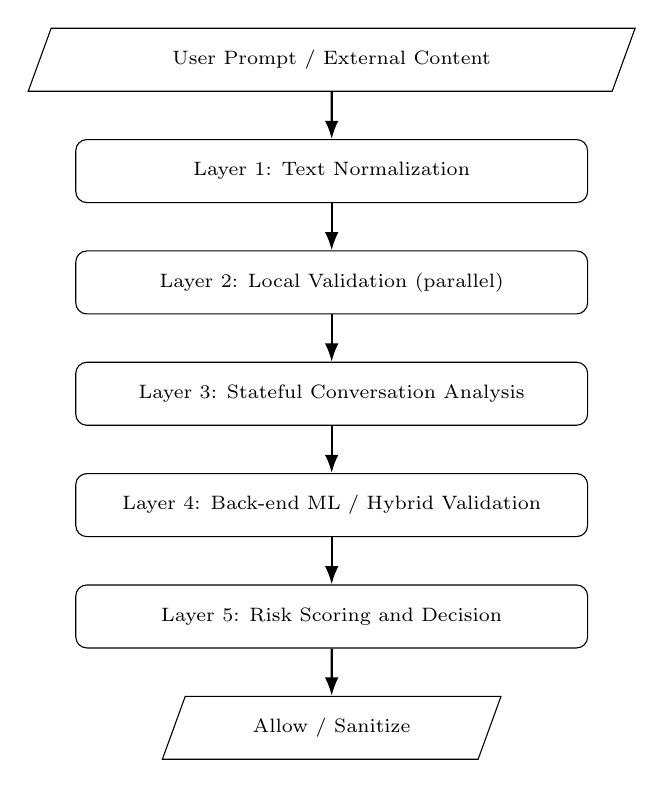
\begin{tikzpicture}[
    font=\scriptsize,
    node distance=6mm,
    box/.style={draw, rounded corners, align=center, minimum width=6.5cm, minimum height=0.8cm},
    data/.style={draw, trapezium, trapezium left angle=70, trapezium right angle=110, align=center, minimum width=4cm, minimum height=0.8cm},
    line/.style={-Latex, thick}
]
\node[data] (input) {User Prompt / External Content};
\node[box, below=of input] (norm) {Layer 1: Text Normalization};
\node[box, below=of norm] (local) {Layer 2: Local Validation (parallel)};
\node[box, below=of local] (context) {Layer 3: Stateful Conversation Analysis};
\node[box, below=of context] (backend) {Layer 4: Back-end ML / Hybrid Validation};
\node[box, below=of backend] (decision) {Layer 5: Risk Scoring and Decision};
\node[data, below=of decision] (out) {Allow / Sanitize};
\draw[line] (input) -- (norm);
\draw[line] (norm) -- (local);
\draw[line] (local) -- (context);
\draw[line] (context) -- (backend);
\draw[line] (backend) -- (decision);
\draw[line] (decision) -- (out);
\end{tikzpicture}
\caption{High-level architecture of Gradril.}
\end{figure}

\section{Actual Request Flow}
The implemented request flow in the extension is as follows:
\begin{enumerate}
    \item receive prompt in the chat participant;
    \item normalize prompt text to reduce obfuscation;
    \item run enabled local validators on normalized text;
    \item optionally call the Guardrails back end if available;
    \item flatten findings and sanitize the original prompt;
    \item compute the risk score and choose either allow or sanitize;
    \item forward the original or sanitized prompt to the model.
\end{enumerate}

A key implementation detail is that the current local decision engine does not perform hard blocking. Instead, it either forwards the original prompt or forwards a sanitized version.

\section{Architectural Contributions}
The architectural novelty of Gradril lies in four design choices. First, normalization is treated as a security layer rather than a preprocessing convenience. Second, detection is decomposed into multiple modules rather than collapsed into a single classifier. Third, a dedicated code-exfiltration detector is introduced for developer-assistant environments. Fourth, a stateful conversation tracker extends security beyond single-turn inspection.

\section{Conclusion of Part I}
Part I established the problem context, prior-work positioning, threat model, and high-level architecture of Gradril. Part II focuses on the concrete low-level implementation, active validators, ML-backed back-end components, and runtime decision behavior.

\end{document}
